\chapter{Prospecting Algorithm}
\label{chapter:prospection}
Prospecting a swarm is one of the key elements of credit mining system. The prospecting module can be divided into two main stage, named early and live prospecting. Both of the stages rely on the swarm measurement by looking at its evolution \cite{2013:swarmevolution:su}. Credit mining system \textit{translates} the peer information it receives to the number of potential seeder and leecher. It also stores the \textit{availability} of the swarm by looking at the pieces possessed by each peers. 

When a swarm is marked as potential source of investment, credit mining system will fetch necessary information of that swarm in \textit{early prospecting stage}. It only executed once and decide whether the swarm is accepted or discarded with a relatively expensive operations. If the swarm accepted and it is possible to get the return of investment, credit mining system activate the \textit{live prospecting stage}. This stage runs continuously with cheap operations for every monitored swarm. The combination of both stages resulting the whole prospecting algorithm. 

\section{Early prospecting stage}

Early prospecting stage is important to decide which swarm that need to be mined. Wrong or sub-optimal decision will lead to low credit to be mined and less effect on the swarm. In a case where the miner decide to choose a particular swarm, then it will optimistically find more information before it switch to another swarm if the decision is not beneficial. This will result with an unnecessary overhead on the miners as a whole.  

The challenge of early prospecting is because we only have very limited, unverified, information of the swarm. In the \bt~nature, there are two ways to get the swarm information : by joining the swarm as peer, or acting as a tracker. Mindlessly download and participate in the swarm may waste the resource we have. Therefore, in the manager, we proposed the procedure called \textit{predownloading}. On top of that, to both tackle the tracker unavailability and get thorough swarm information, \textit{peer translation} mechanism can act as a swarm health predictor.

\begin{algorithm}[h]
	\caption{\textit{Predownload} procedures}
	\label{alg:predown}
	\begin{algorithmic}[1]
		\Function{Predownload}{$infohash$, $n$}
		\If{$|download\_queue| > $ 500}	
		\State recall \Call{PREDOWNLOAD}{$infohash$, $n$}
		\EndIf
		
		\State \Call{push}{$download\_queue$, $infohash$}
		
		\State \Call{set\_pieces}{$infohash$, 0, $n$}
		\State \Call{unset\_pieces}{$infohash$, $n + 1$, \Call{pieces}{$infohash$}}
		
		\State \Call{check\_predownload}{$infohash$}
		\EndFunction
		\Statex
		\Function{check\_predownload}{$infohash$}
		\State $peerlist \gets$ \Call{get\_peers}{$infohash$}
		\State \Call{add\_to\_peerlib}{$peerlist$}
		
		\If{wait long enough $and$ not finished yet}
		\State \Call{pop}{$download\_queue$, $infohash$}
		\State \Return False
		\EndIf
		
		\If{wait long enough $and$ already finished}
		\State \Call{translate\_peer}{\Call{get\_peerlib}{\null}}
		\State \Call{pop}{$download\_queue$, $infohash$}
		\State \Return True
		\EndIf
		
		\If{\Call{is\_complete}{$infohash$}}
		\State mark as finished
		\EndIf
		\State \Call{check\_predownload}{$infohash$}
		\EndFunction		
	\end{algorithmic}
\end{algorithm}

\textit{Predownloading} is a means to download a predefined number of pieces in a particular torrent in such a way that only consumes small portion of resource while trying to get as much information as possible of the swarm. \textit{Predownloading} can run in a different session than the main one so it will not disturb the activity of the main session. Assuming we have $n$ piece to \textit{predownload}. The manager then will just explicitly download the first $n$ piece of a verified torrent and flag it as sequential download activity while reject the rest of the pieces. In this way, instead of occupying a large portion of storage, it only stores those $n$ pieces. While and after \textit{predownloading}, the manager actively ask for new peers to tracker or DHT and store it afterwards. There is a delay introduced when the manager has finished \textit{predownload} all those $n$ pieces. This delay is necessary to give a chance for another peer to response to the manager's query and to request new peer if possible. Pseudocode of this procedures shown in Algorithm \ref{alg:predown}. The mining activity will continue at the point where \textit{predownloading} finished. It will not restart the download from scratch.

To be able to fully decentralized, it is important to not rely on the tracker too much. Although some information we needed can be gathered by querying the tracker, some of the swarms don't have tracker at all. Furthermore, in case of multi-tracker\footnote{Defined in : \url{http://www.bittorrent.org/beps/bep_0012.html}.}, some swarms has entirely different number of seeder and peers for each of the tracker. In figure \ref{fig:diffsr}, it is shown that this problem is very likely to be occurred. Because of this reason, we alternate the swarm information source by looking directly from the connected peers. We called the procedure to interpret swarm information from current and previous connected peers as \textit{peer translating}. 

\begin{figure}[ht]
	\centering
	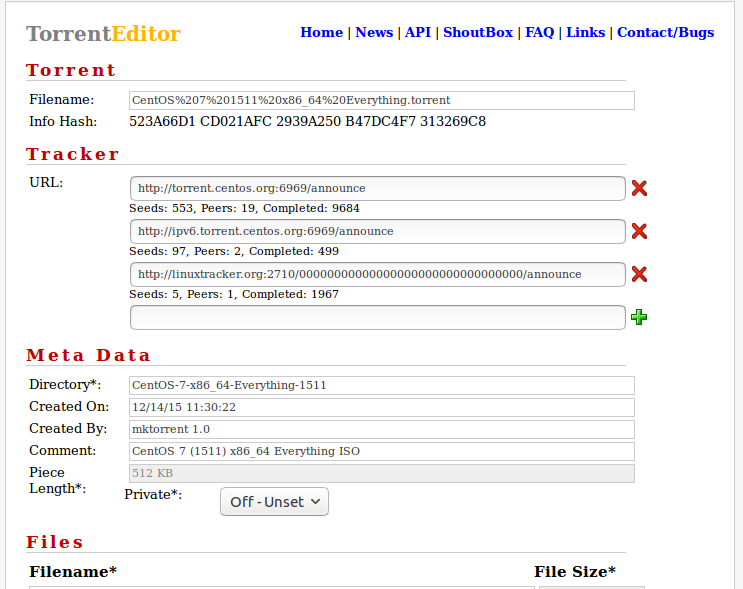
\includegraphics[width=0.8\textwidth]{pics/diffsr.png}
	\caption{Different number of seeder and peers/leecher reported by different trackers.}
	\label{fig:diffsr}
\end{figure}

The \textit{peer translation} receives list of peers as input and returns the number of seeder and downloader. This procedure is shown in Algorithm \ref{alg:peertrans1} and \ref{alg:peertrans2}. The manager will examine each of the peer like shown in \ref{alg:peertrans1}. We categorize a peer is seeder if it satisfy at least one of three conditions. The conditions are: it is only want to upload right now, it is 80\% finished with its download, and it is known to upload more data to us than downloading. In the other hand, we define a peer is a leecher if it satisfies at least one of three conditions, which is: it is interested in our pieces, it has unfinished download and able to download again another piece, and it is known to download more data from us than uploading. We called the phase where the analyzed peers are translated into number of potential seeder and leecher as \textit{interpretation} phase. This phase shown in Algorithm \ref{alg:peertrans2} which is the continuation of Algorithm \ref{alg:peertrans1}.

\begin{algorithm}[t]
	\caption{Peer translation algorithm, analyzing phase}
	\label{alg:peertrans1}
	\begin{algorithmic}[1]
	\Function{translate\_peer}{$peer\_list$}
		\State{$num\_seeder \gets 0$}
		\State{$num\_leecher \gets 0$}
		\Statex
		\State{$upload\_only \gets 0$}
		\State{$finished \gets 0$}
		\State{$unfinished\_able \gets 0$}
		\State{$interested \gets 0$}
		\ForAll{$p \in peer\_list$}
			\If{\Call{upload\_only}{p}}	
			\State $upload\_only \gets upload\_only + 1$
			\EndIf	
			
			\If{\Call{interested}{p}}	
			\State $interested \gets interested + 1$
			\EndIf	
			
			\If{\Call{completed}{p} $>$ 80\%}	
			\State $finished \gets finished + 1$
			\Else
			\If{not \Call{upload\_only}{p}}	
			\State $unfinished\_able \gets unfinished\_able + 1$
			\EndIf	
			\EndIf
		\EndFor
		\algstore{peertranslate}
	\end{algorithmic}
\end{algorithm}

\begin{algorithm}[t]
	\caption{Peer translation algorithm, interpretation phase}
	\label{alg:peertrans2}
	\begin{algorithmic}[1]
		\algrestore{peertranslate}
		\State $num\_seeder \gets $ \Call{max}{$upload\_only$, $finished$}
		\If{$num\_seeder = 0$}	
		\State $num\_seeder \gets $ number of peer who has downloaded bytes $>$ uploaded bytes
		\EndIf
		\State $num\_leecher \gets $ \Call{max}{$interested$, \Call{min}{$unfinished\_able$, $|peer\_list|$ - $finished$}}
		\If{$num\_leecher = 0$}	
		\State $num\_leecher \gets $ number of peer who has uploaded bytes $>$ downloaded bytes
		\EndIf
		\State \Return $num\_seeder$, $num\_leecher$
	\EndFunction
	\end{algorithmic}
\end{algorithm}

\section{Live prospecting}
After the early prospecting has been done, the live prospecting stage will take place regularly. Live prospecting occurred when the credit mining system already decide which swarm that need to be mined.  For a fixed interval, the system evaluates the swarms in \textit{swarm selection} algorithm. It based on \textit{selection policy} which determines the criteria that need to be considered. This policy, however, can not be changed in the runtime.  All the miner need to comply to one defined policy. Swarm with low prospect will be paused, and one with higher prospect replace the old one. Paused swarm may be chosen again in the future. Likewise, the miners may always stick with swarms with very good prospect.

Credit mining system also monitor those swarm continuously, looking for swarm that not well-performed in a particular time frame. This swarm then will be \textit{incited} by optimistically download few rare pieces at one time. The purpose of this approach is to eliminate 

\subsection{Swarm Selection}
Although it is possible for user to create their own policy, three policies have been defined on the preliminary work \cite{2015:creditmining:capota}. Those are based on random, swarm age, and seeder ratio. \textit{Random policy} mostly used as the baseline of the experiment. It is also able to stress test the miners. \textit{Swarm Age policy} is better than random policy. It selects the swarm based on its age. New published swarm known to have higher demand than other type of swarm \cite{2012:economicbt:kash}. Typical user will download a particular item once. Enthusiastic user will download a content as soon as it is published. With a lot of peer in early swarm, it will increase the chance to get more credit. \textit{Seeder Ratio policy} selects the swarm that has lower number of seeder relative to all the peers participated in this swarm. This policy is specialized to help undersupplied swarm. 

\subsection{Scoring Policy}

In this thesis, we intend to extend those policies so it can be highly customizable and cover the balance between gaining credit and helping undersupplied swarm. We propose a policy named \textit{scoring policy} to tackle this issue. Although this policy is more complex than the other basic policies, it is can be customize with several parameters and multipliers of the score. The algorithm of this policy is shown on Algorithm \ref{alg:scorep}. The idea behind this policy is to give higher score for swarm which has lower seeder ratio, has more peers, lower piece availability, and many activities in the swarm. Higher score get higher priority to be mined.

Lower seeder ratio, as mentioned before, is useful to measure whether a swarm is undersupplied or not. This is particularly useful to \textit{help} a swarm. However, in small swarm, this attribute may not be relevant. Thus, a number of peer is considered as a scoring aspect. With the same ratio of seeder and peers, it is useful to mine a big swarm instead of the small one. There are many options to give our piece to. Another important aspect is the file availability of the swarm. In flashcrowd case, there are a significant amount of peer who do not have a large portion of the file. Comparing to another swarm which most of the leecher almost finished their download, mining this swarm will give higher credit and more beneficial to the community altogether. Last element that we considered is the activity of a swarm. It is preferable to mine a swarm whose some of the peers already download or upload any data from or to us. The reason behind this is because the underlying nature of \bt, it is possible that our prediction is wrong. The worst case happened when there are no peer interested with the piece we already have. In the other hand, if a peer already interacted with us before, there is a chance we will get chosen again in the future. Therefore, by putting this attribute into consideration, we want to minimize this problem.

\begin{algorithm}[th]
	\caption{Scoring policy algorithm}
	\label{alg:scorep}
	\begin{algorithmic}[1]
		\Require{$M\_leech$ as leecher multiplier}
		\Require{$M\_pratio$ as peer ratio multiplier}
		\Require{$M\_avail$ as peer availability multiplier}
		\Require{$S\_low$ as score for lower activity}
		\Require{$S\_high$ as score for higher activity}
		\Statex
		\Require{$peerlist$}
		\Require{$swarmlist$}
		\Statex
		\ForAll{$s \in swarmlist$}
			\State{$rleech \gets 1 - $\Call{seeder\_ratio}{s}}
			\State{$rpeer \gets |$\Call{peers}{s}$|/|peerlist|$}
			\State{$ravail \gets 1 - $\Call{availability}{s}$/|peerlist|$}
			\State{$score(s) \gets M\_leech*rleech + M\_pratio * rpeer + M\_avail * ravail$}			\State $total\_speed[s] \gets 0$
			\ForAll{$p \in $\Call{peers}{$s$}}
				\State $total\_speed[s] \gets total\_speed[s] + speed(p)$
			\EndFor
		\EndFor
		\State \Call{sort}{$total\_speed$}
		\ForAll{$s \in swarmlist$}
			\If{$index(total\_speed, s) < |total\_speed|/2$}
				\State $score(s) \gets score(s) + S\_low$
			\Else{\null}
				\State $score(s) \gets score(s) + S\_high$
			\EndIf
		\EndFor
		\State \Return{$score(swarmlist)$}
	\end{algorithmic}
\end{algorithm}

Scoring policy starts with examining all the swarm in a particular miner. Then we decide the score individually as shown in line 2-5. \textit{Peer ratio} is the ratio of a number of peer in this swarm and total number of peers that we know from all the swarm. \textit{Availability} is defined as the number of complete copies of a piece. Non-seeder peer provide a subset of a piece and increase the overall of the availability. In this case, we add the \textit{availability} as the number of peer who has the rarest piece. Moreover, the fraction of piece who has more peer is also considered. It is impossible for \textit{availability} to be 0, as it means there is no one who have complete file. Maximum number of \textit{availability} is the number of peer itself. That means, all the peer has completed files. After the score was assigned, the activity of each peer on each of the swarm is calculated. The activity, stored in a list, is sorted increasingly. Then, first half of the sorted activity is marked as low activity, and given the lower activity score (line 14). Similarly happens with second half of the list, but with higher activity and higher score (line 16).

Scoring policy is intended to be able to facilitate what user need in a simple way. This can be done by providing value to the multiplier. By default, the value of $M\_leech$, $M\_pratio$, and $M\_avail$ are 5, 3, and 4, respectively. We argue that the number of seeder is the most relevant parameter to mine a swarm. Then it is the piece availability and its distribution. In the other hand, we think the the number of peer is less relevant than other parameter. It is indeed important in a case where the number of seeder ratio is exactly the same. Although less relevant, mining a large swarm may increase the probability to meet with potential seeder. That is why we still take it into consideration. In default case, we weight the importance of seeder ratio the most compared to the others. Changing the multiplier also changing the behavior. For example, a user do not consider number of peers important, so he can set the multiplier for $M\_pratio$ as 0. $S\_low$ and $S\_high$ can be configured as well to incentivize swarm who interact with the miner previously.

\subsection{Swarm incitation}

As mentioned in Section \ref{section:sharemode}, activating \textit{share mode} can result in a bottleneck, especially in the beginning of joining a swarm. \textit{Predownload} a swarm, if handled correctly, can solve this issue. It optimistically download a relatively large amount of pieces compared to in share mode algorithm. However, it only run in the initial stage of mining. Moreover, it is not designed to tackle bottlenecked swarm, but to measure the swarm. Therefore, we introduced another method to spur the mining activity. It starts by looking which swarm that already idle for some time. One of the sign a swarm has getting bottleneck can be seen from its activity. To prevent a drop in overall contribution in the swarm, the amount of share ratio is also considered. If this is too low, we should wait for a piece to be uploaded first. And if it is not possible, then this swarm will be blacklisted in the next round anyway. Few rarest pieces will be downloaded from swarms that passed the requirements. All of this process is called \textit{inciting} the swarm. By optimistically download rarest piece simultaneously, we hope to incite the mining activity in the long term.